\section{Semantic Parsing}

\textbf{Goal}: Syntatic Representation => semantic representation. \\ Example: “Everybody loves someone else”: \\ (1) $ \forall p .(\mathrm{Person}(p) \rightarrow \exists q .(\mathrm{Person}(q) \wedge p \neq q \wedge \operatorname{Loves}(p, q)))$, \quad (2) $ \exists p .(\mathrm{Person}(p) \wedge \forall q .(\mathrm{Person}(q) \wedge p \neq q \rightarrow \operatorname{Loves}(q, p)))$

\subsection*{Principle of Compositionality}
(Complex\_expression A).meaning $=$ $f($A.constituents.meanings$)$.

\subsection*{Enriched $\lambda$ calculus to represent meanings}
\textbf{Computation rules}: $\alpha$\textbf{-conversion}: renaming, \\
$\lambda x . \lambda y .(x((\lambda x . x \; x) y)) \rightarrow \lambda z . \lambda y .(z((\lambda x . x \; z) y))$. \\
$\beta$\textbf{-reduction}: applying one lambda term to another, $\lambda y .(z((\lambda \mathbf{x} \cdot \mathbf{x} \; z) y)) \rightarrow \lambda y \cdot(z(z \;y))$.
\vspace{-0.4cm}
\begin{center}
    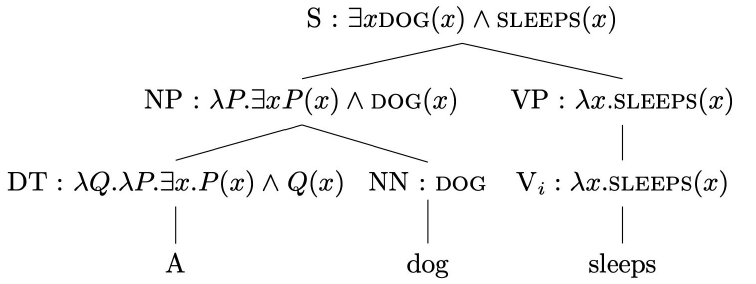
\includegraphics[width=\columnwidth]{img/semantic_representation.png}
\end{center}
\vspace{-0.5cm}
\textit{The semantic form depends on the grammar and combination order.} 

Derivation e.g.: "likes every dog".sem
\vspace{-0.3cm}
\begin{tiny}
\begin{equation*}
    \begin{aligned}
        &=(\mathrm{``likes".sem \;``every dog".sem}) \\
        &=(\lambda P \cdot \lambda Q \cdot Q(\lambda x \cdot P(\lambda y \cdot \operatorname{LIKES}(x, y))) \quad \lambda Q \cdot \forall x(\mathrm{DOG}(x) \Rightarrow Q(x))) \\
        &=(\lambda P \cdot \lambda Q \cdot Q(\lambda t \cdot P(\lambda y \cdot \mathrm{LIKES}(t, y))) \quad \lambda Q \cdot \forall x(\mathrm{DOG}(x) \Rightarrow Q(x))) \\
        &=\lambda Q \cdot Q(\lambda t \cdot(\lambda Q \cdot \forall x(\mathrm{DOG}(x) \Rightarrow Q(x)) \quad(\lambda y \cdot \operatorname{LIKES}(t, y)))) \\
        &=\lambda Q \cdot Q(\lambda t \cdot(\forall x(\mathrm{DOG}(x) \Rightarrow((\lambda y \cdot \mathrm{LIKES}(t, y)) x)))) \\
        &=\lambda Q \cdot Q(\lambda t \cdot(\forall x(\mathrm{DOG}(x) \Rightarrow \mathrm{LIKES}(t, x))))
    \end{aligned}
\end{equation*}
\end{tiny}
\vspace{-0.4cm}
